% This file was created with tikzplotlib v0.10.1.
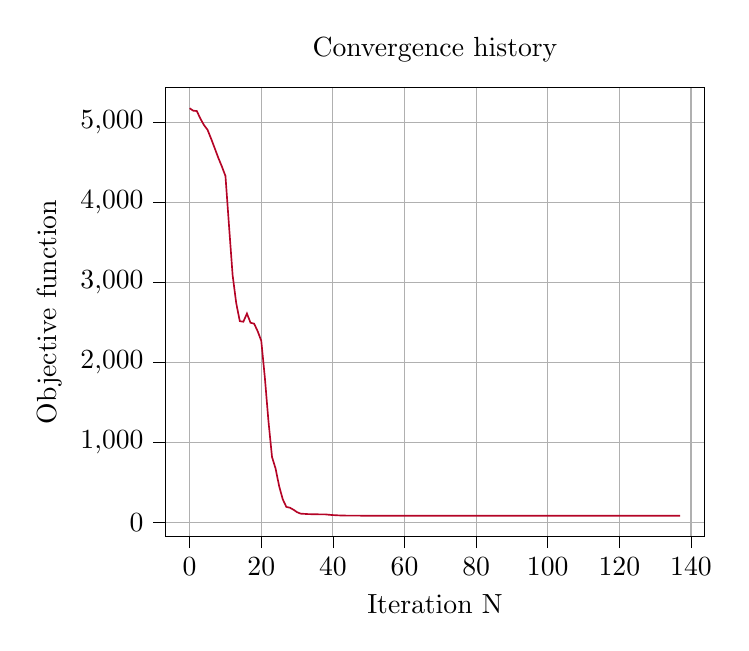
\begin{tikzpicture}

\definecolor{darkgray176}{RGB}{176,176,176}
\definecolor{firebrick180438}{RGB}{180,4,38}

\begin{axis}[
tick align=outside,
tick pos=left,
title={Convergence history},
x grid style={darkgray176},
xlabel={Iteration N},
xmajorgrids,
xmin=-6.85, xmax=143.85,
xtick style={color=black},
y grid style={darkgray176},
ylabel={Objective function},
ymajorgrids,
ymin=-174.13997095568, ymax=5433.41363048767,
ytick style={color=black}
]
\addplot [semithick, firebrick180438]
table {%
0 5178.52483042206
1 5148.03153068576
2 5143.62600246673
3 5048.39254377851
4 4968.17131761947
5 4908.3689122801
6 4797.32516596191
7 4678.92019359868
8 4558.7960034304
9 4449.81787553168
10 4331.2799703791
11 3704.47000785608
12 3090.5353005788
13 2743.23250627881
14 2515.46219332038
15 2508.34095047735
16 2610.73313311735
17 2495.27396982458
18 2484.65736036447
19 2389.18039748159
20 2270.11385809523
21 1810.13308506927
22 1268.44115020189
23 817.480642964819
24 670.751585848601
25 450.292887922839
26 287.410129984884
27 192.289658341375
28 181.892149076243
29 156.915223001589
30 126.472476826756
31 107.715221650914
32 105.173863842041
33 102.355264933656
34 101.06967976509
35 100.164428275714
36 99.2788144265868
37 98.720344472577
38 98.2072999242287
39 93.5708176210384
40 90.2008006702256
41 87.4453525100312
42 85.491463927554
43 84.0329794912388
44 83.4621533827488
45 82.8894838575153
46 83.3527476481473
47 82.8719358230958
48 82.4355842441906
49 82.1116086531509
50 82.0535900678024
51 81.7826061365209
52 81.6997326590713
53 81.642115802854
54 81.6262187469413
55 81.6070725023071
56 81.5760357526757
57 81.5285015645919
58 81.531329599306
59 81.4743577569978
60 81.5558438457995
61 81.6095069245379
62 81.6142992506993
63 81.6221296883003
64 81.6493441753169
65 81.6612102371947
66 81.5005143931175
67 81.4519006800896
68 81.388523562364
69 81.3635544390772
70 81.352996762235
71 81.5987080474373
72 81.5255260058081
73 81.4961172402165
74 81.5262895963655
75 81.5306596043744
76 81.2585595374666
77 81.1466052536568
78 81.045892598657
79 81.0154716836957
80 80.981959376555
81 80.9859000531965
82 80.9815002310546
83 80.9917518863094
84 80.9862876775511
85 80.9874510455015
86 80.9469265177609
87 80.935993543512
88 80.9267902898665
89 80.9246592974015
90 80.9226971187354
91 80.9220569937927
92 80.9216596283576
93 80.9219292911296
94 80.9220796090478
95 80.923496288299
96 80.9234176259863
97 80.9220590462464
98 80.9213743645788
99 80.9209510027686
100 80.9207771346331
101 80.9206684752962
102 80.920480947428
103 80.9200257226525
104 80.9199094853658
105 80.9164531592904
106 80.9157472683053
107 80.9149397585525
108 80.9096193831407
109 80.8990179914538
110 80.8524008088091
111 80.7703673550866
112 80.7542578991824
113 80.7524520590804
114 80.7519915721914
115 80.7488291099269
116 80.7700556934583
117 80.7623640462651
118 80.7811773088236
119 80.7767713180768
120 80.7636876589896
121 80.7678325547683
122 80.760634677547
123 80.7578785993872
124 80.7566871105602
125 80.7584432582076
126 80.7578590837302
127 80.7576283103133
128 80.7575259589639
129 80.7572287399246
130 80.7572512736717
131 80.7556804565862
132 80.755447587514
133 80.7559431796756
134 80.7555810733309
135 80.7556081812871
136 80.7556027353153
137 80.7556058887685
};
\end{axis}

\end{tikzpicture}
